\documentclass[.../main.tex]{subfiles}

\begin{document}

    In this chapter, we summarise and present the research and results which have been obtained thus
    far. These tackle the problems described in Section \ref{sec::Chaos_in_MARL}. We detail the
    derivation of a stability phase line as presented in Sanders et al. \cite{Sanders2018} as well
    as the numerical simulations performed to verify these results. The steps to be completed
    subseqent to this study are then given.

    \section{Convergence and Chaos in Q-Learning Agents} \label{sec::Chaos_in_Q-Learning}

    We begin by considering the evolution of learning with agents who follow a Q-Learning approach.
    Specifically, we look at characterising the stability of agents learning strategies. This
    technique is carried out by Sanders et al \cite{Sanders2018}, in which the authors
    characterise the strategy evolution of agents who learn using an 'Experience Weighted
    Attraction' (EWA) algorithm, which is seen to be a strong representation of how people learn in
    games. The authors are able to determine the regions of parameter space in which learning is
    likely to converge towards stable equilibriums, as opposed to complex behaviours (such as limit
    cycles or chaotic dynamics). The aim of this study is to format these techniques for the study
    of computational agents who follow the popular Q-Learning approach \cite{Sutton2018,SchwartzMulti-agentApproach}.

    We aim, similarly, to determine the regions of parameter space in which the agents are likely to
    converge to stable equilibria. In this way it will be possible to, a priori, determine whether,
    for a particular game, the behaviour is likely to converge and even how to choose the agent or
    game parameters to ensure the predicatability of the resulting behaviour. To achieve this, we
    consult the Q-Learning Dynamics proposed by Tuyls et al \cite{Tuyls2006AnGames}. In this study, the
    authors were able to derive a continuous time dynamical system describing how agents following a
    Q-Learning approach adjust the probabilities of choosing actions as they iteratively play a
    game. These equations are shown in \cite{Tuyls2006AnGames} to accurately model the expected
    behaviour of agents as they iterate a game, and the experiments which verified this model are
    shown in Figures \ref{fig::TuylsExperiments}. 

    With the accuracy of the continuous time dynamical system (\ref{eqn::EOM}) established, we analyse the
    stability of this system in the following section. Note that whilst the derivation provided is
    for the particular case of two agents for the sake of brevity, the problem of p-player games is
    equivalent to that of two players and so the solutions to the former can (and will) be
    presented. 
    
     \subsection{Derivation of stability line} % (fold)
     \label{sub:derivation_of_stability_line}
     
     We begin with the equations as described by Tuyls et al \cite{Tuyls2006AnGames}

    \begin{subequations}
    \label{eqn::EOM}
        \begin{equation}
            \frac{\dot{x}(t)}{x(t)} = \alpha \tau (\sum_{j} a_{ij} y_j - \sum_{i j} x_i a_{ij} y_j)
            + \alpha \sum_j x_j ln(\frac{x_j}{x_i}) 
        \end{equation}
        \begin{equation}
            \frac{\dot{y}(t)}{y(t)} = \alpha \tau (\sum_{j} b_{ij} x_j - \sum_{i j} y_i b_{ij} x_j)
            + \alpha \sum_j y_j ln(\frac{y_j}{y_i}).
        \end{equation}
    \end{subequations}

    Here, $\alpha$ and $\tau$ are the parameters of the agent; Sanders et al. refer to these as the memory and intensity of choice parameters respectively. Agent 1 takes action i with probability $x_i$ while Agent 2 takes action j with probability $y_j$. If these actions are taken, the agents receive payoff $a_{ij}$ and $b_{ji}$ respectively. 

    Our goal is to analyse the dynamics of any game, regardless of payoff elements. As such, we
    follow the approach of Sanders et al. in deriving the full set of 'effective dynamics' averaged
    over all possible realisations of the payoff matrices. Note that these elements are drawn from a
    Multivariate Gaussian such that

    \begin{equation*}
        \begin{split}
            \mathbb{E}[a_{ij}] = \mathbb{E}[b_{ji}] = 0\\
            \mathbb{E}[a_{ij}^2] = \mathbb{E}[b_{ji}^2] = 1\\
            \mathbb{E}[a_{ij} b_{ji}] = \Gamma.
        \end{split}
    \end{equation*}

    where $\Gamma$ is a parameter which defines the 'competitiveness' of the game. For a two player
    game, $\Gamma \in [-1, 1]$ where -1 denotes a zero-sum game and 1 denotes a game with positive
    correlation across payoff elements. Taking this average yields

    \begin{equation}
    \begin{split}
        \dot{x}(t) &= x(t)(\Gamma \alpha^2 \tilde{\tau}^2 \int dt'[G_y(t, t')x(t')] + 
        \tilde{\alpha}
        \rho_x(t) + \alpha \tilde{\tau} \eta_x(t) + \tilde{\alpha} \tau \eta_x(t) \eta_y(t) +
        \sqrt{\Gamma} \tilde{\alpha} \tau \mu_x) \\
        \dot{y}(t) &= y(t)(\Gamma \alpha^2 \tilde{\tau}^2 \int dt'[G_x(t, t')y(t')] + 
        \tilde{\alpha} \rho_y(t) +
        \alpha \tilde{\tau} \eta_y(t) + \tilde{\alpha} \tau \eta_x(t) \eta_y(t)+ 
        \sqrt{\Gamma} \tilde{\alpha} \tau \mu_y), \\
    \end{split}
    \end{equation}

    Here, $G, \rho, \eta, \mu$ are correlation functions, generated due to the averaging process 
    and the notation $\tilde{\cdot}$ denotes a term which has been scaled with respect to $N$ (see
    Appendix \ref{app::ResearchSummary} for method and notation). We now analyse the stability of
    this dynamical system by linearising about a fixed point. This yields the requirement that a
    fixed point $x^*$ satisfy

    \begin{equation}
    0 = x^* \left[\Gamma \alpha^2 \tilde{\tau}^2 x^* \int G_y(t - t') dt' + \tilde{\alpha} \rho_x^* + \alpha \tilde{\tau} \eta_x^* + \tilde{\alpha} \tau \eta_x^* \eta_y^* + \sqrt{\Gamma} \tilde{\alpha} \tau \mu_x \right].
    \end{equation}

    The implication here is that the resulting value of $x^*$ can take two solutions. However, one
    of these is $x^* = 0$, which is found to rarely occur \cite{Coolen2005}, while the second solution
    contains a term $\sqrt{\Gamma}$, which would yield complex values. Such a result, of course, is
    not possible for a quantity denoting probabilities and so it appears that the theory cannot hold
    for $\Gamma < 0$. However, numerical experiments will shed light on the likelihood of
    convergence and the islands of stability in parameter space for this region.

    We take the Fourier transform of this system to determine the long term behaviour of the system
    after a disturbance. To neglect all transient behaviour (high frequency disturbances), we
    consider the equation at $\omega = 0$

    \begin{equation} \label{eqn::Transformed}
    \left<[|\mathcal{X}(\omega)|^2 \right> = \left< | \Gamma \alpha \tilde{\tau} \mathcal{V}_x(\omega) + \tilde{\alpha} \tau \eta^*_x \mathcal{V}_y(\omega) + \tilde{\alpha} \tau \eta^*_y \mathcal{V}_x(\omega) + \sqrt{\Gamma} \tilde{\alpha} \tau \Delta(\omega) + \Xi(\omega) |^2 \right> \frac{1}{\left< |\mathcal{A}(\omega, x^*) |^2 \right>}, 
    \end{equation}


    where

    \begin{equation}
        \mathcal{A}(\omega, x^*) = \frac{i \omega}{x^*} - \Gamma \alpha^2 \tilde{\tau}^2 \mathcal{G}_y(\omega)
    \end{equation}

    By
    considering that $\left<|\mathcal{X}(\omega =
    0)|^2
    \right> \geq 0$  we arrive at an expression for a stability line (i.e. the phase transition
    between the
    existence of stable fixed points and unstable behaviour) as the equality (\ref{eqn::Transformed}
    )$>0$.

    % subsection derivation_of_stability_line (end)

    \subsection{Numerical Experiments} % (fold)
    \label{sub:numerical_experiments}
    
    To verify the results of our theory, and to examine the underlying structure of stability and
    chaos in Multi-Agent Q Learning, we perform a series of numerical experiments by varying the
    parameters $\Gamma$ and $\alpha$ whilst keeping $\tau$ fixed. This yields the result shown in
    Figure \ref{fig::NumericalExperiments}. We see from this, and from the further experiments shown
    in Appendix \ref{app::ResearchSummary}, that the stability of the system is highly dependent on
    the value of $\tau$.
    For
    low values, the system converges almost everywhere, whilst increasing $\tau$ to 0.15 decreases
    the probability of convergence significantly.

    \begin{figure}[h]
        \centering
         \begin{subfigure}[b]{0.45 \textwidth}
        \centering
        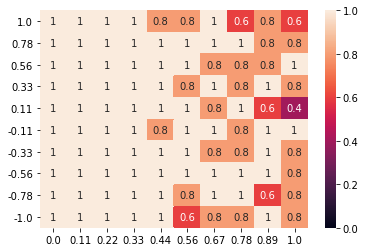
\includegraphics[width = 0.7 \textwidth]{Figures/AlphaRun_tau_005.png}
        \caption{$\tau = 0.05$}
        \end{subfigure}
        \begin{subfigure}[b]{0.45 \textwidth}
        \centering
        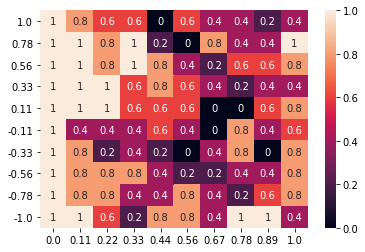
\includegraphics[width = 0.7 \textwidth]{Figures/tau_015.png}
        \caption{$\tau = 0.15$}
        \end{subfigure}

        \caption{$\alpha = 0.1$, $\gamma = 0.1$, $\tau \in [0.1, 10]$, $\Gamma \in [-1, 1]$. Each
        simulation is run for 1e5 iterations and tested for convergence. The game is said to have
        converged based on a tolerance of 1\% difference between action probabilities. For each
        combination of $\tau$, $\Gamma$ the game is played 5 times, each with random payoff matrices
        and initial conditions. The average number of converged games (giving an indication of
        probability of convergence) is shown in each cell of the heatmap. 
        \label{fig::NumericalExperiments}}
    \end{figure}

   To generate the numerical simulations in Figure \ref{fig::NumericalExperiments} we used the
   following procedure.

\begin{enumerate}
    \item Fix the parameters $\alpha$ and $\gamma$. The latter is held fixed at $0.1$ since
    it does not affect the long term behaviour of the system (it does not appear in (
    \ref{eqn::EOM})).
    \item We initialise values of $\Gamma$ and $\tau$. These will be the variables which we sweep
    over.
    \item Generate payoff matrices for both agents by sampling from a multi-variate Gaussian 
    (variables are the payoff elements) with covariance parameterised by $\Gamma$.
    \item Initialise the agents with random initial conditions (i.e. random action probabilities).
    \item Allow the agents to learn over a maximum of $1 \times 10^5$ iterations.
    \item Every 100 iterations, check to see if the action probabilities have changed significantly.
    If not (i.e. the change over the last 100 iterations is less than 1\%) the learning is
    considered to have converged.
    \item This process is repeated 5 times with random payoff matrices generated based on the value
    of $\Gamma$. The probability of convergence is then recorded as $\frac{\text{number of times
    converged}}{5}$.
    \item The values of $\tau$ and $\Gamma$ are then modified and the process is repeated. The
    heatmap shows the probability of convergence for all values of $\tau$ and $\Gamma$ which are
    tested.
\end{enumerate}

    % subsection numerical_experiments (end)

    \subsection*{Future Work} \label{sec::Future Work}

    We are currently running a set of numerical experiments varying over all three parameters
    $\Gamma, \alpha, \tau$ to identify any islands of stability in parameter space. We will then
    plot (\ref{eqn::Transformed}) to verify our results.

    As mentioned, the above system considers only a two player game. This was done with the intention
    of simplifying the notation and reducing the complexity of the experiments. However, the next
    immediate action is to present the equivalent solutions for the case of a general $p$-player
    game.
    
    We then seek to expand this study to a population of agents. For this, we will study the
    stability of the system presented by Leung et al \cite{Hu2019} which presents a mean-field model
    describing the evolution of learning of a population of Q-Learning agents who play co-operative
    games against one another. This last point is an important limitation - the derived dynamics
    will only consider populations who must co-operate with one another (i.e. the $\Gamma$ value of
    the game is one). 

\end{document}